\documentclass[11pt,a4paper]{article}
%%%%%%%%%%%%%%%%%%%%%%%%%%%%%%%%%%%%%%%%%%%%%%%%%%%%%%%%
%                      PACKAGES                        %
%%%%%%%%%%%%%%%%%%%%%%%%%%%%%%%%%%%%%%%%%%%%%%%%%%%%%%%%

\usepackage[utf8]{inputenc}
\usepackage{graphicx} % Allows you to insert figures
\usepackage[export]{adjustbox}
\usepackage{booktabs}
\usepackage{amsmath} % Allows you to do equations
\usepackage{helvet}
\usepackage{hyperref}
\renewcommand{\familydefault}{\sfdefault}
\usepackage[a4paper, total={6.5in, 9.5in}]{geometry} % Formats the paper size, orientation, and margins
\linespread{1.1} % about 1.5 spacing in Word
\setlength{\parindent}{0pt} % no paragraph indents
\setlength{\parskip}{1em} % paragraphs separated by one line
\usepackage{listings}
\usepackage{enumitem}
\usepackage{xcolor}
\usepackage{hyperref}
\hypersetup{
	colorlinks=true,
	urlcolor=cyan,
	linktoc=none,
}
\usepackage{fancyhdr}
\pagestyle{fancy}
\fancyhead[L,C,R]{}
\fancyfoot[L]{Occupi - Office Capacity Predictor}
\fancyfoot[C]{}
\fancyfoot[R]{\textbf{\thepage}}
\renewcommand{\headrulewidth}{0pt}
\renewcommand{\footrulewidth}{0.5pt}

\definecolor{codegreen}{rgb}{0,0.6,0}
\definecolor{codegray}{rgb}{0.5,0.5,0.5}
\definecolor{codepurple}{rgb}{0.58,0,0.82}
\definecolor{backcolour}{rgb}{0.95,0.95,0.92}

\lstdefinestyle{mystyle}{
backgroundcolor=\color{backcolour},
commentstyle=\color{codegreen},
keywordstyle=\color{magenta},
numberstyle=\tiny\color{codegray},
stringstyle=\color{codepurple},
basicstyle=\ttfamily\footnotesize,
breakatwhitespace=false,
breaklines=true,
keepspaces=true,
numbers=left,
numbersep=5pt,
showspaces=false,
showstringspaces=false,
showtabs=false,
tabsize=2,
}

\lstset{style=mystyle}
\def\code#1{\texttt{#1}}

%%%%%%%%%%%%%%%%%%%%%%%%%%%%%%%%%%%%%%%%%%%%%%%%%%%%%%%%
%            TITLE PAGE & TABLE OF CONTENTS            %
%%%%%%%%%%%%%%%%%%%%%%%%%%%%%%%%%%%%%%%%%%%%%%%%%%%%%%%%

\begin{document}

\begin{titlepage}
    \centering
    % \includegraphics[width=0.5\textwidth]{your_logo.png}\par\vspace{1cm}
    {\scshape\LARGE Software Requirements Specification\par}
    \vspace{1.5cm}
    {\huge\bfseries Occupi - Office Capacity Predictor\par}
    \vspace{2.5cm}
    \begin{tabular}{|c|c|}
        \hline
        \textbf{Name}      & \textbf{Student Number} \\
        \hline
        Rethakgetse Manaka & u22491032               \\
        Kamogelo Moeketse  & u22623478               \\
        Michael Chinyama   & u21546551               \\
        Tinashe Austin     & u21564176               \\
        Carey Mokou        & u21631532               \\
        \hline
    \end{tabular}
    \vfill
    {\large June 24, 2024\par}
\end{titlepage}

\tableofcontents
\pagebreak

%%%%%%%%%%%%%%%%%%%%%%%%%%%%%%%%%%%%%%%%%%%%%%%%%%%%%%%%
%                MAIN DOCUMENT CONTENT                 %
%%%%%%%%%%%%%%%%%%%%%%%%%%%%%%%%%%%%%%%%%%%%%%%%%%%%%%%%

\section*{Introduction}
\addcontentsline{toc}{section}{Introduction}
The Occupi-Office Capacity Management system is designed to revolutionize the way office space is managed by integrating advanced Machine Learning and predictive models. This innovative system addresses the challenge of efficiently managing office occupancy by providing real-time updates on the current capacity and predicting future occupancy trends.

By leveraging historical data and real-time inputs, the Occupi system enables office managers to make informed decisions about space utilization. It not only provides immediate insights into current occupancy levels but also offers longer-term predictions, facilitating better planning and allocation of resources. This planning capability allows the system to enhance its predictive accuracy over time, creating a dynamic and responsive tool for office capacity management.

The system benefits both daily users and office owners. Employees and visitors can access real-time updates on the current office capacity, ensuring they are aware of occupancy levels before arriving. Office managers and owners receive detailed predictions on future capacity, empowering them to optimize space usage, plan for peak periods, and enhance overall office efficiency.

In summary, the Occupi-Office Capacity Management system introduces a data-driven approach to managing office space, offering both immediate and long-term solutions to enhance occupancy management and improve office operations.

\section*{Purpose and Vision}
\addcontentsline{toc}{section}{Purpose and Vision}
The Occupi-Office Capacity Management system aims to revolutionize office space management by integrating advanced Machine Learning and predictive models. The system addresses the challenge of efficiently managing office occupancy by providing real-time updates on current capacity and predicting future occupancy trends. This enables office managers to make informed decisions about space utilization, ensuring optimal use of office resources.

The vision of the Occupi-Office Capacity Management system is to create a dynamic and responsive tool that benefits both daily users and office owners. By leveraging historical data and real-time inputs, the system offers immediate insights into current occupancy levels and detailed predictions for future capacity. This facilitates better planning and resource allocation, allowing the system to enhance its predictive accuracy over time. Ultimately, the system seeks to introduce a data-driven approach to office capacity management, improving office operations and space efficiency.

\pagebreak

\section*{Specifications}
\addcontentsline{toc}{section}{Specifications}

\subsection*{System Requirements}
\addcontentsline{toc}{subsection}{System Requirements}
Occupi is compatible with the following operating systems:
\begin{itemize}
    \item Windows
    \item Linux
    \item MacOS
    \item Android
    \item iOS
\end{itemize}
Internet connection is required for the system to function optimally.

\pagebreak

\section*{User Stories and Characteristics}
\addcontentsline{toc}{section}{User Stories and Characteristics}

\subsection*{Characteristics}
\addcontentsline{toc}{subsection}{Characteristics}
\paragraph{Employees}
Employees are the primary users of the Occupi-Office Capacity Management system. Their main goal is to efficiently manage their work schedules by leveraging real-time occupancy data and predictions.
\begin{itemize}
    \item \textbf{Check-In:} Employees want to use the app to check in when they arrive at the office, providing the system with accurate occupancy data.
    \item \textbf{View Current Office Capacity:} Employees want to use the system to quickly view the current number of people in the office through the app, helping them decide when to come in or find a less crowded time.
    \item \textbf{Plan Visits:} By accessing occupancy predictions, employees want to plan their visits around expected busy times, enhancing their productivity and ensuring a comfortable working environment.
    \item \textbf{Notifications and Alerts:} Employees want to receive notifications about significant changes in occupancy or office conditions, such as reaching maximum capacity or scheduled maintenance.
\end{itemize}

\paragraph{Managers}
Managers use the Occupi system to make strategic decisions regarding office space utilization and to ensure a smooth operation of the office environment. Managers want to manage their teams effectively and optimize office resources.
\begin{itemize}
    \item \textbf{Historical Trends:} Managers want to access detailed historical data on office occupancy, helping them identify patterns and trends over time.
    \item \textbf{Space Planning:} Using predictions and historical data, managers want to plan the allocation of office space, schedule shifts, and manage peak times effectively.
    \item \textbf{Reporting:} Managers want to generate reports on office usage, occupancy trends, and space efficiency to inform higher-level strategic decisions.
    \item \textbf{Team Management:} Managers want to generate reports on team attendance rates, productivity, and collaboration patterns, helping them optimize team performance and office layout.
\end{itemize}

\paragraph{System Administrators}
System Administrators are responsible for maintaining the overall functionality, data integrity, and performance of the Occupi system.
\begin{itemize}
    \item \textbf{Data Accuracy:} Administrators want to ensure that the data collected by the sensors and other devices is accurate and reliable.
    \item \textbf{System Performance:} Administrators want to monitor system performance, addressing any issues that arise and ensuring that the application runs smoothly.
    \item \textbf{Security:} Administrators want to manage the security of the system, including user access controls, data encryption, and compliance with relevant data protection regulations.
    \item \textbf{Maintenance and Updates:} They perform regular maintenance and updates to the system, ensuring it remains up-to-date with the latest features and security patches.
    \item \textbf{Technical Support:} Provide technical support to other users, troubleshooting issues and providing guidance on using the system effectively.
\end{itemize}

\paragraph{General Staff}
General Staff such as facility management or administrative staff use the system to manage the physical aspects of the office environment.
\begin{itemize}
    \item \textbf{Room Booking for Cleaning:} General Staff want to book specific rooms for cleaning through the system, ensuring that all areas are properly maintained without disrupting employees.
    \item \textbf{Maintenance Scheduling:} General Staff want to schedule and manage maintenance activities, disabling rooms or areas as needed to perform repairs or upgrades.
    \item \textbf{Notifications:} General Staff want to receive notifications about required maintenance or cleaning tasks, allowing them to manage their workload effectively.
    \item \textbf{Resource Management:} General Staff want to oversee the allocation and usage of office resources, such as cleaning supplies and maintenance tools, based on occupancy data and predictions.
\end{itemize}

\pagebreak

\subsection*{Stories}
\addcontentsline{toc}{subsection}{Stories}
\paragraph{Employees}
\begin{itemize}
    \item As an employee, I want to log in using my credentials to access the Occupi system.
    \item As an employee, I want to check in when I arrive at the office to update the occupancy data.
    \item As an employee, I want to see the real-time office capacity so that I can decide whether to come to the office.
    \item As an employee, I want to view predicted office capacity for the next two days so that I can plan my office visits accordingly.
    \item As an employee, I want to update my profile information so that my contact details and preferences are accurate.
    \item As an employee, I want to receive notifications about office capacity updates so that I am informed if the office is full.
    \item As an employee, I want to provide feedback on the app so that the development team can improve it.
    \item As an employee, I want to navigate the app easily so that I can find information quickly.
    \item As an employee, I want to use the application in my preferred language so that I can navigate it easily.
    \item As an employee, I want to search for occupancy data by date so that I can find specific information quickly.
    \item As an employee, I want to be able to report issues with rooms or facilities so that they can be addressed promptly.
\end{itemize}

\paragraph{Managers}
\begin{itemize}
    \item As a manager, I want to view historical occupancy data so that I can identify trends and patterns.
    \item As a manager, I want to generate reports on office occupancy so that I can make informed decisions.
    \item As a manager, I want to receive alerts about office capacity changes so that I can respond quickly.
    \item As a manager, I want to view team attendance rates so that I can optimize team performance.
    \item As a manager, I want to export occupancy data so that I can analyze it externally or share it with stakeholders.
    \item As a manager, I want to search for occupancy data by date so that I can quickly retrieve specific information for analysis or reporting.
    \item As a manager, I want to receive feedback on the app from users so that I can understand user needs and improve the application.
    \item As a manager, I want to receive a daily summary report of office occupancy so that I can review daily trends.
    \item As a manager, I want to see visual representations of historical data so that I can understand trends better.
\end{itemize}

\paragraph{System Administrators}
\begin{itemize}
    \item As a system administrator, I want to monitor system performance so that I can identify and address issues.
    \item As a system administrator, I want to manage user access controls so that I can ensure data security.
    \item As a system administrator, I want to update the system regularly so that it remains secure and up-to-date.
    \item As a system administrator, I want to receive alerts about system issues so that I can respond quickly.
    \item As a system administrator, I want to provide technical support to users so that they can use the system effectively.
    \item As a system administrator, I want to manage data encryption so that user data is secure.
    \item As a system administrator, I want to view audit logs of check-ins and check-outs so that I can track user actions for security purposes.
    \item As a system administrator, I want to integrate the app with building access control systems so that check-in data is automatically updated.
    \item As a system administrator, I want to set capacity alert thresholds so that I am notified when occupancy reaches critical levels.
\end{itemize}

\paragraph{General Staff}
\begin{itemize}
    \item As general staff, I want to book rooms for cleaning through the system so that I can manage cleaning schedules effectively.
    \item As general staff, I want to schedule maintenance activities through the system so that I can plan maintenance tasks efficiently.
    \item As general staff, I want to receive notifications about required maintenance or cleaning tasks so that I can manage my workload effectively.
\end{itemize}

\pagebreak

\section*{Class Diagrams}
\addcontentsline{toc}{section}{Class Diagrams}
% Include your class diagrams here using 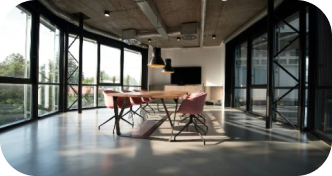
\includegraphics{path/to/your/image}

\clearpage

\pagebreak

\section*{Functional Requirements}
\addcontentsline{toc}{section}{Functional Requirements}

\subsection*{Requirements}
\addcontentsline{toc}{subsection}{Requirements}
Requirements with a \textbf{*} next to it represents optional and \textit{nice to have} requirements.

\begin{enumerate}[label=\arabic*.]
    \item Provide a secure authentication process.
    \item Users must be able to log in using their credentials.
    \item Users must be able to log in using their Deloitte email address and password.
    \item Users must be able to log out of the system.
    \item Users must be able to reset their password.
    \item Users onboard using an OTP that expires after 10 minutes.
    \item Provide a user-friendly interface.
    \item Users must be able to navigate the app easily.
    \item Users must be able to search for information quickly.
    \item Users must be able to use the app in their preferred language.
    \item Users must be able to choose between different themes: 'Light' and 'Dark'.
    \item Provide real-time office capacity updates.
    \item Users must be able to check in when they arrive at the office.
    \item Users must be able to view the current office capacity.
    \item Users must be able to receive notifications about office capacity updates.
    \item Provide office capacity predictions.
    \item Users must be able to view predicted office capacity for the next two days.
    \item Users must be able to plan their office visits accordingly.
    \item Provide historical occupancy data.
    \item Managers must be able to view historical occupancy data.
    \item Managers must be able to identify trends and patterns.
    \item Managers must be able to generate reports on office occupancy.
    \item Generate reports on office occupancy.
    \item Managers must be able to generate reports on office occupancy for the past week.
    \item Managers must be able to generate reports on office occupancy for the past month.
    \item Managers must be able to generate reports on office occupancy for the past year.
    \item Managers must be able to generate reports on team attendance rates.
    \item Managers must be able to generate reports on team attendance rates for the past week.
    \item Managers must be able to generate reports on team attendance rates for the past month.
    \item Managers must be able to generate reports on team attendance rates for the past year.
    \item Managers must be able to generate reports on team attendance rates for a specific individual.
    \item Managers must be able to generate reports on team attendance rates for a specific date.
    \item Manage user access controls.
    \item System administrators must be able to manage user access controls.
    \item System administrators must be able to specify user roles.
    \item System administrators must be able to assign users to specific roles.
    \item System administrators must be able to revoke user access.
    \item System administrators must be able to set capacity alert thresholds.
    \item System administrators must be able to ensure data security.
    \item Provide booking functionality.
    \item Users must be able to book specific rooms for specific time periods.
    \item Users must be able to view room availability.
    \item Users must be able to cancel bookings.
    \item Users must be able to invite other users to join booking room.
    \item Provide Check-in functionality.
    \item Users must be able to check in for a specific booking.
    \item Users must be able to check in using booking details and credentials.
    \item System must detect that users are checking from a specific location.
    \item System must implement automatic check out.
    \item Provide maintenance scheduling.
    \item General staff must be able to schedule maintenance activities through the system.
    \item General staff must be able to book rooms for cleaning through the system.
    \item Provide notifications.
    \item Users must be able to receive notifications about maintenance taking place.
    \item Users must be able to receive notifications about office capacity updates.
    \item Users must be able to receive notifications about their bookings.
\end{enumerate}

\subsection*{Subsystems}
\addcontentsline{toc}{subsection}{Subsystems}
\begin{enumerate}
    \item User Management
    \item Profile Management
    \item Predictive Model to graph
    \item Security Management
    \item Room Management
    \item Analytics and Reporting
\end{enumerate}

\pagebreak

\subsection*{Use Case Diagrams}
\addcontentsline{toc}{subsection}{Use Case Diagrams}

\subsubsection*{Profile Management Subsystem}
\begin{figure}[htbp]
    \centering
    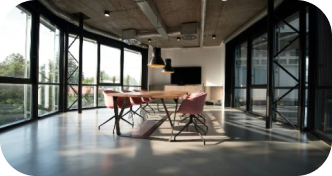
\includegraphics[width=1\textwidth]{path/to/your/image}
\end{figure}

\pagebreak
\subsubsection*{User Management Subsystem}
\begin{figure}[htbp]
    \centering
    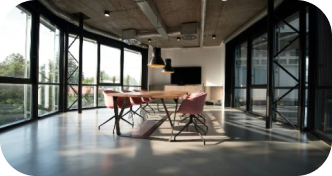
\includegraphics[width=1\textwidth]{path/to/your/image}
\end{figure}

\subsubsection*{Room Management Subsystem}
\begin{figure}[htbp]
    \centering
    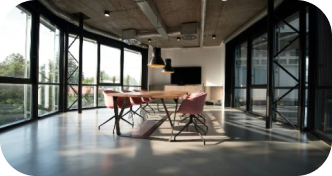
\includegraphics[width=1\textwidth]{path/to/your/image}
\end{figure}

\pagebreak

\section*{Quality Requirements}
\addcontentsline{toc}{section}{Quality Requirements}

\subsection*{Performance}
The performance of the Occupi system is critical to its success. The system will be accessed by a large number of users and it must be able to handle high traffic loads without slowing down or crashing. The system should respond quickly to user requests, providing real-time updates on office capacity and occupancy predictions. To ensure optimal performance, the system should be able to scale horizontally to accommodate additional users and data. The system should also be able to handle peak loads during busy periods, such as the start and end of the workday. Performance testing should be conducted regularly to identify and address any bottlenecks or issues that may arise.

\subsection*{Reliability}
The reliability of the Occupi system is essential to ensure that users can access the system when they need it. The only time that is acceptable for the system to be down is during maintenance. To ensure reliability, the system should be designed with redundancy and failover mechanisms to prevent downtime. Regular backups of data should be performed to prevent data loss in the event of a system failure. Data should be backed up every 7 days and be recoverable within 24 hours. The system should also be monitored for performance and availability, with alerts sent to administrators if any issues are detected.

\subsection*{Scalability}
The Occupi system should be able to scale to accommodate additional users, data, and features as needed. The architecture of the system should be designed to support horizontal scaling. This means that additional servers can be added to the system to handle increased traffic and data without affecting performance. The system should also be able to scale vertically, allowing individual components to be upgraded to handle increased load.

\subsection*{Security}
The security of the Occupi system is paramount to protect user data and ensure the integrity of the system. Due to the system collecting data on users, it is important that the system is secure. The system should implement strong encryption to protect data in transit and at rest. User authentication should be implemented to ensure that only authorized users can access the system. Access controls should be in place to restrict user access to sensitive data and features. User authentication should take place every 90 days. User authentication systems such as OAuth should be implemented to ensure that user data is secure. Domain-specific access should be implemented to ensure that only users with the correct domain can access the system.

\subsection*{Usability}
The Occupi system should be easy to use and navigate, with an intuitive interface that allows users to find information quickly and easily. The system should be accessible and user-friendly, with clear instructions and guidance provided to help users understand how to use the system. The system should follow Deloitte design cues and be consistent across all platforms. The system should also be responsive, adapting to different screen sizes and devices to provide a consistent user experience. User feedback should be collected regularly to identify areas for improvement and enhance the usability of the system.

\subsection*{Interoperability}
The Occupi system should integrate seamlessly with Deloitte’s building access control system. This allows the system to automatically update occupancy data based on user check-ins and check-outs. The system should also be compatible with a wide range of devices and platforms, including desktops, laptops, tablets, and smartphones. The system should also integrate with the building’s network infrastructure to ensure that users are checking in from the correct location. The system should be able to keep track of trends in the Deloitte tuckshop by integrating with the tuckshop system.

\subsection*{Compliance}
Due to personal data being collected, the Occupi system must comply with relevant data protection regulations, such as the Protection of Personal Information Act (POPIA). The system should implement data protection measures to ensure that user data is secure and protected from unauthorized access. The system should also comply with industry standards and best practices for data security and privacy. Regular audits and reviews should be conducted to ensure that the system remains compliant with Deloitte’s data protection policies and relevant regulations.

\subsection*{Compatibility}
The Occupi system should be compatible with a wide range of devices and platforms, including desktops, laptops, tablets, and smartphones. The system should be accessible from any device with an internet connection, allowing users to access real-time updates on office capacity and occupancy predictions. The system must be compatible with the following operating systems:
\begin{itemize}
    \item Windows
    \item Linux
    \item MacOS
    \item Android
    \item iOS
\end{itemize}

\pagebreak

\section*{Design Strategy}
\addcontentsline{toc}{section}{Design Strategy}
The architectural design strategy for the development of Occupi involves the following: Agile and Decomposition.

\subsection*{Agile Strategy}
This strategy focuses on iterative development, continuous feedback from clients, cross-functional teams, as well as adaptability. Iterative development involves work being divided into small, manageable increments. This aids the development process of the project in that it allows the team to break parts of the projects apart and focus on one part at a time. This makes the project more manageable. Continuous feedback from the client helps to ensure that the product meets their needs. This helps to prevent the team from diverting from the requirements of the product.

\subsection*{Decomposition Strategy}
This strategy emphasizes breaking down complex projects into smaller, more manageable components. Decomposition involves dividing the project into discrete, self-contained modules or tasks. This approach enhances the development process by allowing the team to concentrate on individual segments, making the overall project easier to handle. Each module can be developed, tested, and refined independently before integrating it into the larger system. Regular assessments and adjustments at each stage ensure that each part aligns with the overall project goals. This strategy minimizes risks, improves resource allocation, and ensures that the final product meets the desired standards and specifications.

\pagebreak

\section*{Architectural Design \& Patterns}
\addcontentsline{toc}{section}{Architectural Design \& Patterns}
\subsection*{MVC (Model-View-Controller)}
We chose the MVC to separate concerns for user interface, business logic, and data management. The MVC pattern promotes a clean separation of concerns between data management (Model), user interface (View), and application logic (Controller), making our codebase more modular and easier to maintain.

\textbf{Model: Database} - The Model represents the core backend of our system, managing the data and the business logic. It serves as the central source of truth for all other views in the system. In our architecture, the Model includes:
\begin{itemize}
    \item \textbf{MongoDB:} The primary database for storing and retrieving application data. MongoDB's NoSQL structure allows for flexible, scalable, and high-performance data management.
\end{itemize}

\textbf{View: Frontend} - The View is responsible for displaying data to the user and capturing user input. It is the user interface layer of the application. In our architecture, the View includes:
\begin{itemize}
    \item \textbf{Web Frontend (React):} The client-side part of the application for our Management Terminal, built using React. It renders the user interface, allowing users to interact with the system. It displays dashboards and other data visualization elements to assist in understanding office capacity trends.
    \item \textbf{Mobile Frontend (React Native):} The client-side part of the application for mobile users, built using React Native. It provides a seamless and responsive user experience on mobile devices whilst booking, checking in, and viewing office occupancy.
\end{itemize}

\textbf{Controller: AI Model Server} - The Controller acts as an intermediary between the Model and the View. It processes incoming requests, performs operations on the Model, and updates the View accordingly. In our architecture, the Controller includes:
\begin{itemize}
    \item \textbf{Python AI Model:} Integrates AI-related operations such as data processing, making predictions, and providing intelligent responses. This component works closely with the Go server to handle AI tasks.
\end{itemize}

\subsection*{Layered Pattern}
\begin{itemize}
    \item \textbf{Presentation Layer:} This layer consists of the user interfaces such as the mobile application for employees and the management terminal for managers. It handles user input, displays data, and provides a consistent user experience adhering to Deloitte's design standards and guidelines (Usability and Compliance).
    \item \textbf{Application Layer:} This layer encapsulates the business logic and rules related to occupancy tracking, prediction algorithms, and other core functionalities of the system. It serves as an intermediary between the Presentation Layer and the lower layers, ensuring proper separation of concerns.
    \item \textbf{Service Layer:} This layer consists of various services or components responsible for specific tasks such as user management, occupancy tracking, prediction engine, and real-time updates. These services could be implemented as microservices, promoting scalability and maintainability.
    \item \textbf{Data Access Layer:} This layer abstracts the underlying data storage mechanisms (e.g., MongoDB) and provides a consistent interface for interacting with the data sources. It handles tasks such as querying, updating, and retrieving data related to occupancy, historical trends, and user information.
    \item \textbf{External Systems Layer:} This layer facilitates integration with external systems such as Deloitte's existing building access control systems. It handles communication protocols, data transformations, and any necessary adaptations required for seamless integration (Interoperability).
    \item \textbf{Security Layer:} This layer handles authentication, authorization, and other security-related concerns such as encryption and data protection (Security). It could be implemented as a cross-cutting concern or as a separate layer depending on the complexity of the security requirements.
\end{itemize}

\subsection*{Client Server}
\textbf{Client:} The client in this instance acts as any vector that forwards requests to the backend. Clients can access the server from multiple endpoints and different environments including that of production and development environments. Our domain registrar handles DNS for the clients and forwards requests to the IP address of the server.

\textbf{Server:} We have a singular VM instance that acts as a server which listens for incoming requests on port 443 (HTTPs) and serves clients multiple different pages depending on what URL they sent in. A client may be served our documentation site, the landing page, the actual web app, or the API backend (which may interact with the database) which are all hosted in containers. A reverse proxy sits between port 443 and our containers.

\pagebreak

\section*{Technology Choices}
\addcontentsline{toc}{section}{Technology Choices}
\subsection*{For Web-based Development}
\paragraph{React:} A JavaScript library for building user interfaces. It's component-based which promotes reusability and makes code easier to manage. However, the learning curve can be steep for beginners.
\begin{itemize}
    \item \textbf{Pros:}
          \begin{itemize}
              \item Component-based architecture allows for modular and reusable code.
              \item Large ecosystem with a vast array of libraries and tools.
              \item Virtual DOM for efficient rendering and updates.
              \item Supported by a large community and backed by Facebook.
          \end{itemize}
\end{itemize}

\paragraph{Tailwind CSS:} A utility-first CSS framework that allows for highly customizable designs. It can speed up development, but the class-based approach might seem verbose to some.
\begin{itemize}
    \item \textbf{Pros:}
          \begin{itemize}
              \item Utility-first approach allows for rapid styling and prototyping.
              \item Highly customizable and flexible.
              \item Promotes consistency and maintainability across projects.
          \end{itemize}
\end{itemize}

\paragraph{Component libraries (Schadcn, DaisyUI, NextUI, Framer Motion):} These libraries provide pre-built components that can speed up development and ensure consistency across the app. However, they might limit customization to some extent.
\begin{itemize}
    \item \textbf{Pros:}
          \begin{itemize}
              \item Accelerates development by providing pre-built UI components.
              \item Ensures consistent design and styling across the application.
              \item Well-documented and actively maintained by communities.
          \end{itemize}
\end{itemize}

\subsection*{For Mobile Development}
\paragraph{React Native:} A framework for building native apps using React. It allows for code sharing between platforms which can reduce development time. However, it might not be as performant as native code for complex applications.
\begin{itemize}
    \item \textbf{Pros:}
          \begin{itemize}
              \item Write once, run anywhere (iOS and Android) with native performance.
              \item Large community and extensive ecosystem of libraries and tools.
              \item Easier learning curve for developers familiar with React.
          \end{itemize}
\end{itemize}

\paragraph{Component libraries (UI Kitten, GlueStackUI):} Similar to web development, these libraries can speed up development and ensure consistency. The same potential limitation in customization applies.
\begin{itemize}
    \item \textbf{Pros:}
          \begin{itemize}
              \item Pre-built components specifically designed for React Native.
              \item Consistent look and feel across platforms.
              \item Actively maintained and well-documented.
          \end{itemize}
\end{itemize}

\subsection*{Reasons for Frontend}
We chose React for our project due to its component-based architecture which promotes modular and reusable code and its efficient rendering capabilities via the Virtual DOM. Tailwind CSS was selected for its utility-first approach, enabling rapid styling and prototyping with high customizability and consistency. Additionally, component libraries like Schadcn, DaisyUI, NextUI, and Framer Motion offer pre-built components that accelerate development and maintain a consistent design across the app, despite some limitations in customization. This combination of tools provides a robust and efficient development environment backed by a large community and extensive ecosystem.

\subsection*{For Backend Development}
\paragraph{Go:} A statically typed, compiled language that is efficient and excellent for building web services and microservices. However, its simplicity can be a limitation for some complex applications.
\begin{itemize}
    \item \textbf{Pros:}
          \begin{itemize}
              \item Statically typed language which promotes code safety and reliability.
              \item Excellent performance and high concurrency support.
              \item Simple and clean syntax, easy to learn and maintain.
              \item Built-in support for concurrency and parallelism.
          \end{itemize}
\end{itemize}

\paragraph{MongoDB driver support:} This allows for rapid development and deployment, especially for web services, microservices, and cloud-native apps. However, MongoDB might not be the best choice for applications that require complex transactions with multiple operations.
\begin{itemize}
    \item \textbf{Pros:}
          \begin{itemize}
              \item Supports a flexible and scalable NoSQL database.
              \item Enables rapid development and deployment of web services and microservices.
              \item Well-suited for cloud-native applications and distributed systems.
              \item Requires a different mindset and approach compared to traditional relational databases.
          \end{itemize}
\end{itemize}

\paragraph{REST API, JSON Web Tokens:} REST is a standard for designing networked applications. It can be simpler and more scalable than other approaches, but it might not be as real-time as some applications require. JSON Web Tokens provide a secure way of transmitting information between parties. However, they can be vulnerable if not handled properly.
\begin{itemize}
    \item \textbf{Pros:}
          \begin{itemize}
              \item REST APIs provide a standard and widely adopted architectural style for building web services.
              \item JWTs offer a compact and secure way to transmit claims between parties.
              \item Stateless authentication mechanism reducing server-side overhead.
          \end{itemize}
\end{itemize}

\subsection*{Reasons for Backend}
For backend development, we selected Go due to its statically typed nature which promotes code safety and reliability. Go's excellent performance, high concurrency support, and simple clean syntax make it ideal for building web services and microservices. Its built-in support for concurrency and parallelism further enhances its efficiency. We also chose MongoDB for its flexible and scalable NoSQL database capabilities, enabling rapid development and deployment, especially for web services, microservices, and cloud-native applications. Additionally, we opted for REST API and JSON Web Tokens (JWTs) for their simplicity, scalability, and secure way of transmitting information. REST APIs provide a standard architectural style for building web services, while JWTs offer a compact, secure, and stateless authentication mechanism reducing server-side overhead.

\section*{Architectural Design}
\addcontentsline{toc}{section}{Architectural Design}
% Include your architectural design here using 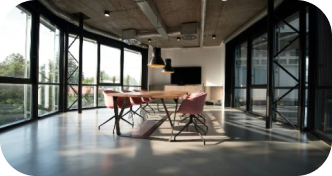
\includegraphics{path/to/your/image}

\end{document}
